\documentclass{beamer}
\mode<presentation> {
%\usetheme{default}
\usetheme{Madrid}


% As well as themes, the Beamer class has a number of color themes
% for any slide theme. Uncomment each of these in turn to see how it
% changes the colors of your current slide theme.
%\usecolortheme{albatross}


%\setbeamertempla
%\titlegraphic{\includegraphics[width=5cm]{assets/cinna.jpeg}}
\title[KDE近似]{KDE近似} % The short title appears at the bottom of every slide, the full title is only on the title page

\author{师清} % Your namete{footline} % To remove the footer line in all slides uncomment this line
%\setbeamertemplate{footline}[page number] % To replace the footer line in all slides with a simple slide count uncomment this line
%\setbeamertemplate{navigation symbols}{} % To remove the navigation symbols from the bottom of all slides uncomment this line
}



%\pgfdeclareimage[height=1.57cm]{university-logo}{assets/cinna.jpeg}
%\logo{\pgfuseimage{university-logo}}

\usepackage{tikz}
\usepackage{graphicx} % Allows including images
\usepackage{booktabs} % Allows the use of \toprule, \midrule and \bottomrule in tables
\usepackage{ctex}
%\usepackage{pythonhighlight}
\usepackage{minted}
\usepackage{hyperref}
\hypersetup{
	colorlinks=true,
	linkcolor=blue,
	filecolor=magenta,      
	urlcolor=cyan,
	pdftitle={Overleaf Example},
	pdfpagemode=FullScreen,
}

%----------------------------------------------------------------------------------------
%	TITLE PAGE
%----------------------------------------------------------------------------------------
\institute[FDU]{FDU}
\date{\today} % Date, can be changed to a custom date

\begin{document}
\begin{frame}
	\titlepage % Print the title page as the first slide
\end{frame}

%Overview frame
\begin{frame}
	\frametitle{Overview} % Table of contents slide
	\tableofcontents % Throughout your presentation, if you choose to use \section{} and \subsection{} commands, these will automatically be printed on this slide as an overview of your presentation
	\begin{itemize}
		\item 问题定义
		\item paper:《large-scale nonconvex optimization:randomization,gap estimation and numerical resolution》
		\begin{itemize}
			\item Relaxation by randomization
			\item Selection method
			\item Frank-Wolfe Algorithm 
		\end{itemize}

	\end{itemize}
\end{frame}

\begin{frame}{问题定义:kde近似}
\begin{align}
	& f(x) = \sum_{i=1}^{N_1}w_i^{'}exp\left[-\frac{(x-p_i)^2}{h}\right] \nonumber \\
	& x_j \sim f(x) \rightarrow \left\{x_j\right\}_M \nonumber \\
	& g(x) = \sum_{i=1}^{N_2}w_iexp\left[-\frac{(x-q_i)^2}{h}\right] \nonumber
\end{align}
\end{frame}

\begin{frame}{问题定义:kde近似}
	\begin{align}
	& \Vert f(x)-g(x) \Vert_2^2 \nonumber\\
	& \approx  \sum_{j=1}^{M} \left( f(x_j)- g(x_j) \right)^2\nonumber \\
	& = \sum_{j=1}^{M}\left(t_j-g(x_j)  \right)^2\nonumber \\
	& = \sum_{j=1}^{j=M}\left\{\sum_{i=1}^{N}w_iexp\left[-\frac{(x_j-q_i)^2}{h}\right]-t_j\right\}^2\nonumber\\
	& = \sum_{j=1}^{j=M}\left\{\sum_{i=1}^{N}w_iexp\left[-\frac{(y_j-x_i)^2}{h}\right]-t_j\right\}^2 \nonumber
	\end{align}
\end{frame}

\begin{frame}{二次规划}
	\begin{align}
	 &\sum_{j=1}^{j=M}\left\{\sum_{i=1}^{N}w_iexp\left[-\frac{(y_j-x_i)^2}{h}\right]-t_j\right\}^2 \nonumber \\
	 &=  \sum_{j=1}^{j=M}\left\{\sum_{i=1}^{N}w_ia_{ji}-t_j\right\}^2 \nonumber\\
	 & =  \Vert A\mathbf{w}-\mathbf{t} \Vert_2^2  \nonumber \\
	 & = (A\mathbf{w}-\mathbf{t} )^T(A\mathbf{w}-\mathbf{t} ) \nonumber \\
	 & = \mathbf{w}^TA^T A\mathbf{w}-2\mathbf{t}^TA\mathbf{w}  \nonumber\\
	 & = \frac{1}{2}\mathbf{w}^TQ\mathbf{w}+\mathbf{b}^T\mathbf{w}  \nonumber \\
	 &constraints:\mathbf{1}^T\mathbf{w}=1 , \mathbf{w} \ge 0 \nonumber
	\end{align}
\end{frame}


\begin{frame}{问题定义:kde近似}

\begin{align}
	& inf_{x\in \mathcal{X}} J(x):=f(G(x))=f(\frac{1}{N}\sum_{i=1}^{N}g_i(x_i))=\sum_{j=1}^{M}f_j(\frac{1}{N}\sum_{i=1}^{N}g_{ij}(x_i)) \nonumber \\
		&inf_{\mu \in P_{\delta}} \mathcal{J}(x):=f(\frac{1}{N}\sum_{i=1}^{N}E_{\mu_i}\left[g_i\right])=\sum_{j=1}^{M}f_j(\frac{1}{N}\sum_{i=1}^{N}E_{\mu_i}\left[g_{ij}\right]) \nonumber 
\end{align}
\begin{itemize}
	\item Relaxation by randomization:repalce each optimization variable $x_i$ by a probability measure $\mu_i$, $g_i(x_i)$ are replaced by their integral with respect to $\mu_i$, $E_{\mu_i}\left[g_i\right]$.
	\item Selection method: simulate N
	independent random variables $(X_1 ...  X_N )$, with distributions $X_i \sim \mu_i$
	\item Frank-wolfe algorithm:solve randomized problem
\end{itemize}
\end{frame}

\begin{frame}{Notations}

	\begin{align}
		& S_{ij}:=\left\{g_{ij}(x_i)|x_i\in \mathcal{X}\right\} \quad and\quad S_j:=\frac{1}{N}S_{ij}\nonumber \\
		&C_1 = \sum_{j=1}^{M}\left(L_j \mathop{max}\limits_{1\le i \le N} \left\{d_{ij}\right\}\right) \quad and \quad C_1 = \frac{1}{N}\sum_{j=1}^{M}\left(\widetilde{L}_j \mathop{max}\limits_{1\le i \le N} \left\{d_{ij}\right\}\right) \nonumber
	\end{align}
		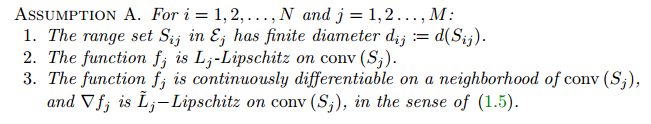
\includegraphics[width=\textwidth]{kde/0.png}
\end{frame}



\begin{frame}{Relaxation by randomization}
	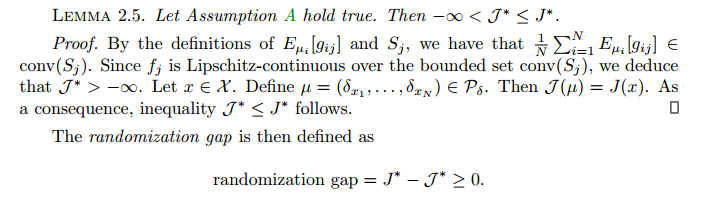
\includegraphics[width=\textwidth]{kde/1.png}
\end{frame}

\begin{frame}{Relaxation by randomization}
	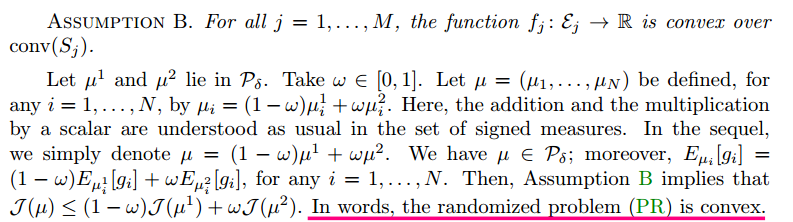
\includegraphics[width=\textwidth]{kde/18.png}
\end{frame}

\begin{frame}{Relaxation by randomization}
	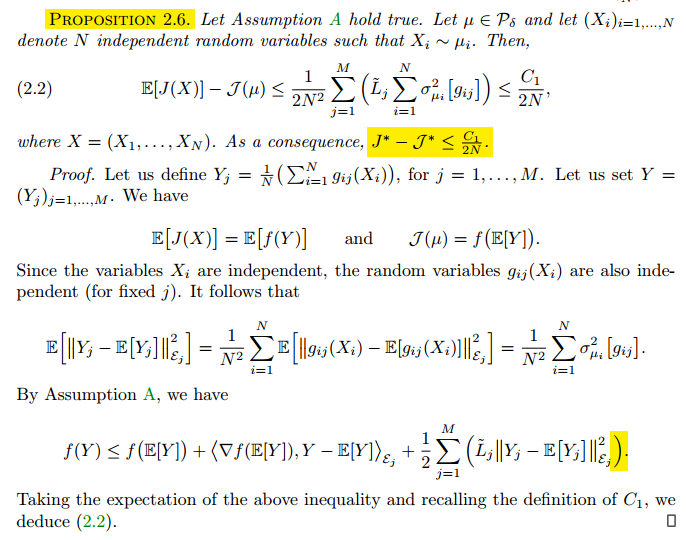
\includegraphics[width=0.8\textwidth]{kde/2.png}
\end{frame}



\begin{frame}{Relaxation by randomization}
	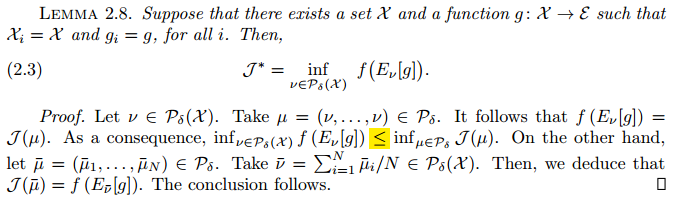
\includegraphics[width=\textwidth]{kde/3.png}
\end{frame}

\begin{frame}{Selection method}
	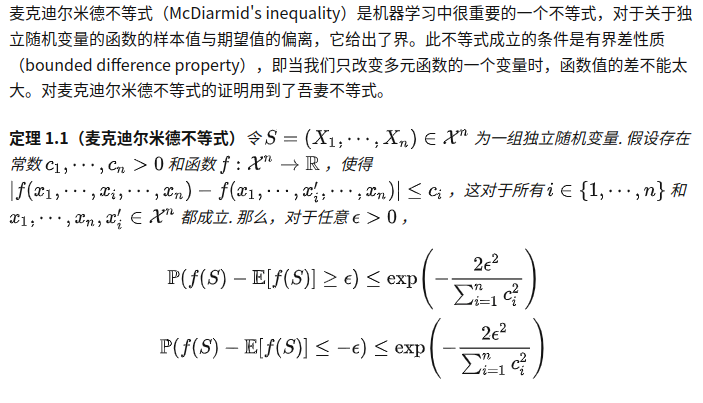
\includegraphics[width=\textwidth]{kde/5.png}
\end{frame}

\begin{frame}{Selection method}
	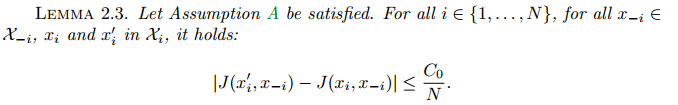
\includegraphics[width=\textwidth]{kde/15.png}
\end{frame}

\begin{frame}{Selection method}
	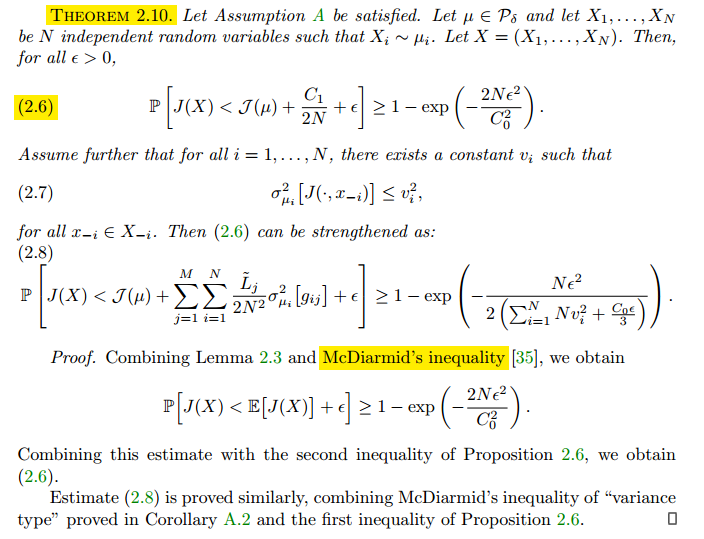
\includegraphics[width=0.9\textwidth]{kde/4.png}
\end{frame}

\begin{frame}{Selection method}
	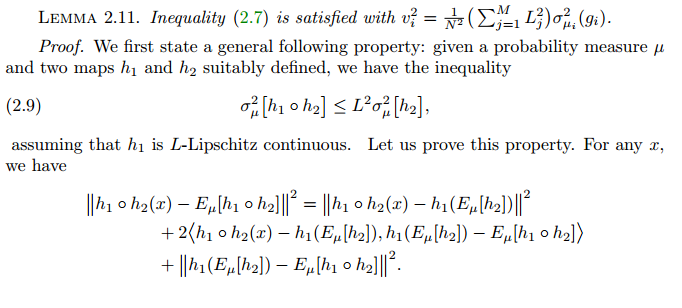
\includegraphics[width=0.8\textwidth]{kde/16.png}
	\\
		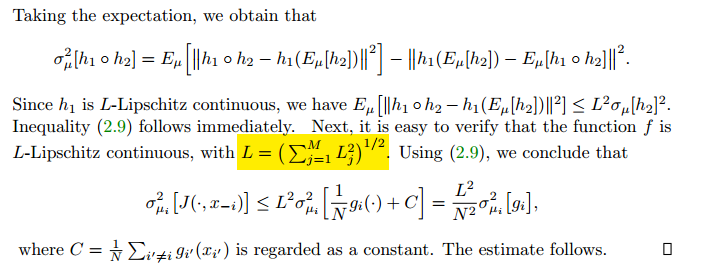
\includegraphics[width=0.8\textwidth]{kde/17.png}
\end{frame}

\begin{frame}{Frank-Wolfe algorithm}
	\begin{align}
		Define:\mathcal{A}:=\left\{\nabla f(y)|y\in conv(G(\mathcal{X}))\right\} \nonumber
	\end{align}
	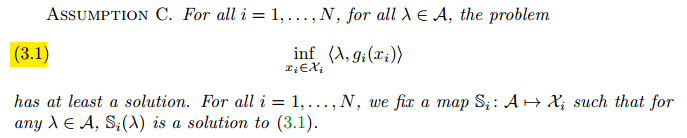
\includegraphics[width=\textwidth]{kde/6.png}
	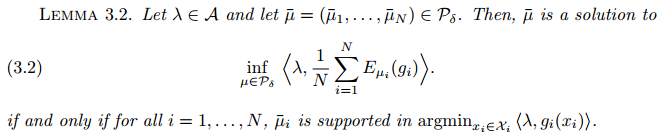
\includegraphics[width=\textwidth]{kde/7.png}
\end{frame}

\begin{frame}{Frank-Wolfe algorithm}
	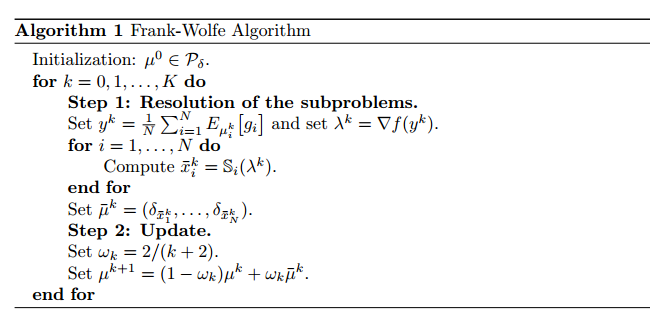
\includegraphics[width=\textwidth]{kde/8.png}
\end{frame}

\begin{frame}{Frank-Wolfe algorithm}
	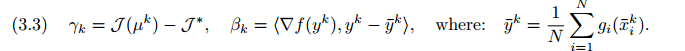
\includegraphics[width=\textwidth]{kde/9.png}\\
	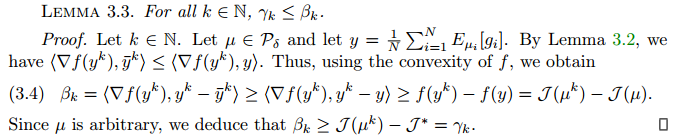
\includegraphics[width=\textwidth]{kde/10.png}
\end{frame}



\begin{frame}{Frank-Wolfe algorithm}
	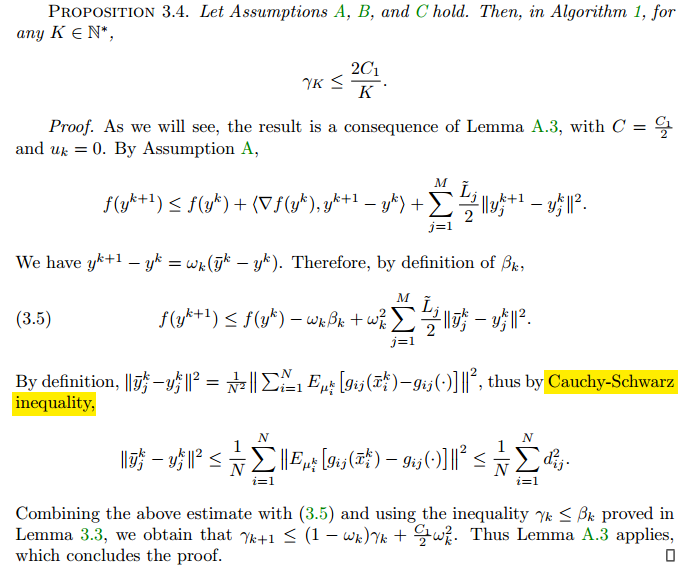
\includegraphics[width=0.8\textwidth]{kde/11.png}
\end{frame}

\begin{frame}{Frank-Wolfe algorithm}
	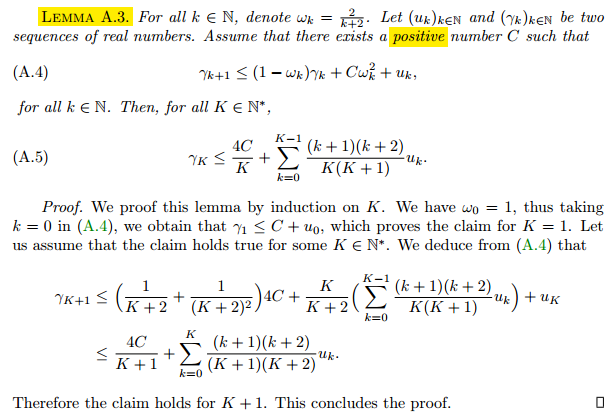
\includegraphics[width=0.8\textwidth]{kde/19.png}
\end{frame}

\begin{frame}{Frank-Wolfe algorithm}
	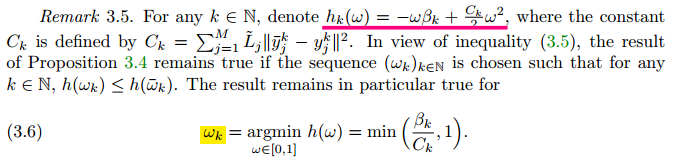
\includegraphics[width=\textwidth]{kde/13.png}
\end{frame}

\begin{frame}{{Frank-Wolfe algorithm}}
	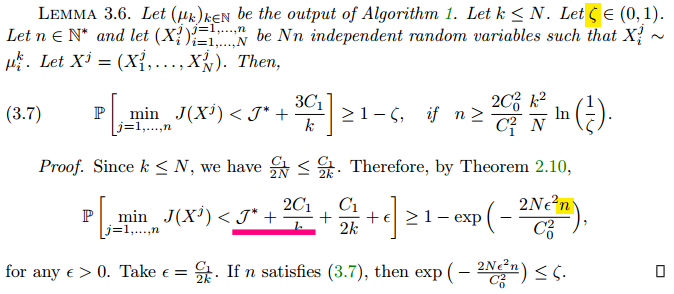
\includegraphics[width=\textwidth]{kde/12.png}
\end{frame}

\end{document} 
